\subsection{ArbIS}
\label{analysis_processing_correlation_arbis_matched}
As with the congestion - accident datasets in \cref{analysis_processing_correlation_baysis_matched,analysis_processing_correlation_baysis_initiator,analysis_processing_correlation_baysis_effector,analysis_processing_correlation_baysis_follower} the congestion - roadwork dataset also needs to be analyzed for correlations. The correlation matrix table for the congestion-roadwork dataset (see \cref{tbl:appendix_arbis_correlation_matrix_dataset_cramers}) is visual presented in \cref{img:correlation_matrix_arbis_selected_effector_cramers} showing the the correlation of each variable combination. When visual analyzing \cref{img:correlation_matrix_arbis_selected_effector_cramers} and checking the guidelines for a strong correlation in reference to the applied coefficient (identifiable with \cref{table:appendix_coefficient_matrix_matched}) we get a list of strongly correlated variable combinations (see \cref{tbl:correlation_list_arbis_matched}). Since the focus of the thesis are the correlations between accidents and jams, these are only collected from the bottom-left rectangle of the matrix, where the congestion and accidents variables intersect. Correlations of the kind congestion - congestion or roadwork - roadwork are not considered.
\begin{table}[h!]
	\centering
	\begin{tabular}{c|l|l}  
		Category & Strong \\
		\\[-1em]
		\hline
		\\[-1em]
		Strasse & TMax, TAvg, SMax, SAvg, TDist, SDist, Cov, TLCar, TLHGV \\ 
 		%AnzGesperrtFs & & \\ 
 		%Einzug & & \\
 		%Richtung & & \\
 		%Length & & \\
 		%Duration & & \\
 		Month & TAvg, SMax, SAvg, TDist, SDist, Cov, TLCar \\
	\end{tabular}
  \caption{List of incident variables and their strong/moderated correlated jam variable from the ArbIS matched data}
  \label{tbl:correlation_list_arbis_matched}
\end{table}
As \cref{tbl:correlation_list_arbis_matched} show, only the variables Strasse and Month are correlated with congestion characteristics. Both variables tend to bias an interpretation of congestion characteristics because the 


Next we need to verify that the correlation is significant and what the correlation predicates. Therefore each correlation will be evaluated with the Post Hoc test, defined in \cref{correlation_posthoc}. In the following sections, the correlated relations of the variables in \cref{tbl:correlation_list_arbis_matched} are analyzed and an initial interpretation of each significant correlation is introduced. Groups with an insufficient sample size (see \cref{correlation_uncertainty} are neglected and not shown. The descriptive tables, showing the count ($n$), mean ($\bar{x}$), standard deviation ($\sigma$), median ($\tilde{x}$), $min$, $max$ and range ($\Delta$) therefore only contain groups with significant sample sizes.
\begin{figure}[!ht]
	\centering
	\makebox[\textwidth][c]{%
		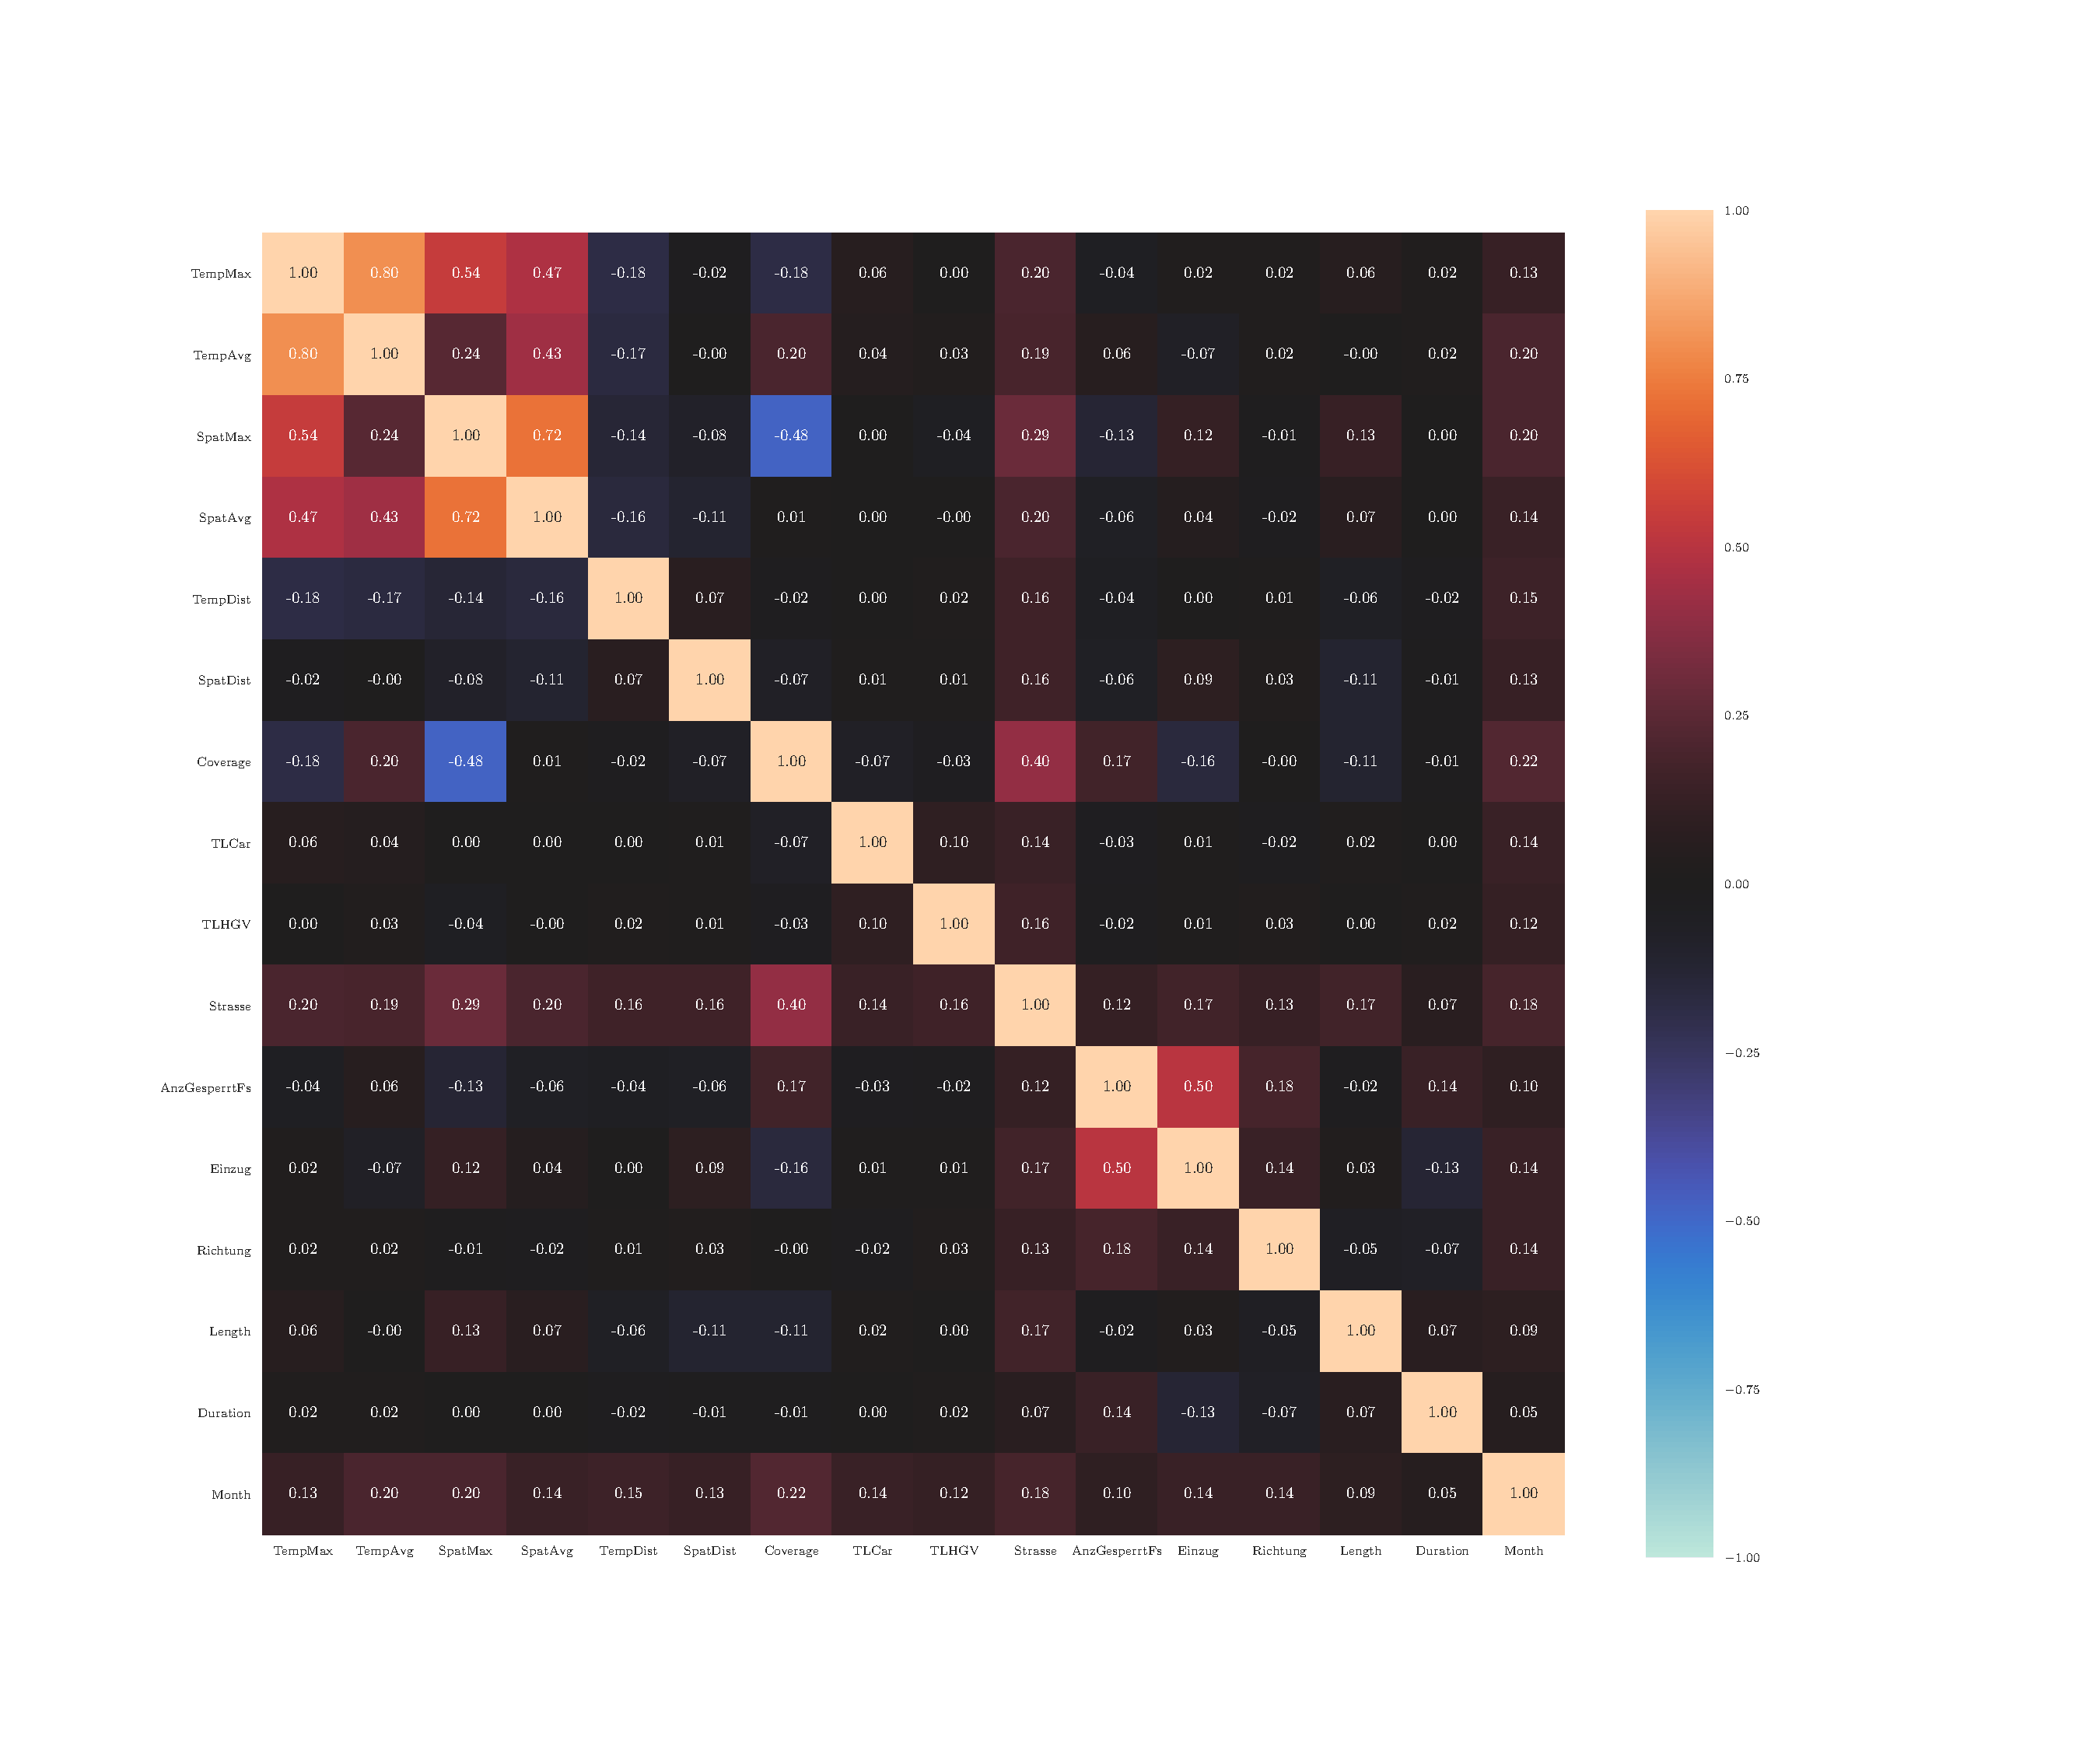
\includegraphics[width=1.4\textwidth, trim=0cm 2.5cm 6cm 3cm]{CorrAnalysis/data/ArbIS/02_matched/plots/arbis_matched_corr_cramers}%
	}
	\caption{Correlation matrix for congestion-roadwork matched data, calculated with $V$, $\eta$, $\tau$, $r_{pq}$, $r$}
	\label{img:correlation_matrix_arbis_selected_effector_cramers}
\end{figure}

% % --------------------------
% % -------- Strasse ---------
% % --------------------------
\centerheading{Strasse}
This section analyzes the correlated relations of the accident variable \textit{Strasse}. The Kruskal-Wallis rank sum test of \textit{Strasse} - \textit{TMax} produces a $p$-value of < 0.0001, which is below $\alpha$. The null hypothesis can therefore be rejected, which means there is a significant difference between the groups of \textit{Strasse}. To identify the significant groups, a pairwise Wilcoxon $T$-test for \textit{Strasse} - \textit{TMax} is run, which produces \cref{tbl:wilcoxon_arbis_matched_Strasse_TMax}. 
\begin{table}[ht!]
	\tiny
	\centering
    \begin{tabular}{rrrrrrrrrrrrrrrrr}
		\toprule
			& A9 & A7 & A70 & A71 & A6 & A73 & A3 & A99 & A96 & A995 & A92 & A72 & A93 & A95 & A94 & A980 \\ 
		\midrule
		% A7   & 1.00 &  &  &  &  &  &  &  &  &  &  &  &  &  &  &  \\ 
		% A70  & 1.00 & 1.00 &  &  &  &  &  &  &  &  &  &  &  &  &  &  \\ 
		% A71  & 1.00 & 1.00 & 1.00 &  &  &  &  &  &  &  &  &  &  &  &  &  \\ 
		% A6   & 1.00 & 1.00 & 1.00 & 1.00 &  &  &  &  &  &  &  &  &  &  &  &  \\ 
		% A73  & 1.00 & 1.00 & 1.00 & 1.00 & 1.00 &  &  &  &  &  &  &  &  &  &  &  \\ 
		A3   & \red{0.00} & \red{0.04} & 1.00 & 1.00 & \red{0.01} & 1.00 &  &  &  &  &  &  &  &  &  &  \\ 
		% A99  & 1.00 & 1.00 & 1.00 & 1.00 & 0.48 & 1.00 & 1.00 &  &  &  &  &  &  &  &  &  \\ 
		A96  & 1.00 & 0.82 & 1.00 & 1.00 & 1.00 & 1.00 & \red{0.00} & \red{0.00} &  &  &  &  &  &  &  &  \\ 
		% A995 & 1.00 & 1.00 & 1.00 & 1.00 & 1.00 & 1.00 & 0.79 & 0.74 & 1.00 &  &  &  &  &  &  &  \\ 
		% A92  & 1.00 & 1.00 & 1.00 & 1.00 & 1.00 & 1.00 & 1.00 & 1.00 & 1.00 & 1.00 &  &  &  &  &  &  \\ 
		% A72  & 1.00 & 1.00 & 1.00 & 1.00 & 1.00 & 1.00 & 1.00 & 1.00 & 1.00 & 1.00 & 1.00 &  &  &  &  &  \\ 
		A93  & \red{0.00} & \red{0.00} & 1.00 & 0.09 & \red{0.00} & \red{0.00} & 1.00 & 1.00 & \red{0.00} & \red{0.00} & \red{0.00} & 1.00 &  &  &  &  \\ 
		% A95  & 1.00 & 1.00 & 1.00 & 1.00 & 1.00 & 1.00 & 1.00 & 1.00 & 1.00 & 1.00 & 1.00 & 1.00 & 1.00 &  &  &  \\ 
		A94  & 1.00 & 1.00 & 1.00 & 1.00 & 0.68 & 1.00 & 1.00 & 1.00 & \red{0.01} & 0.48 & 1.00 & 1.00 & 1.00 & 1.00 &  &  \\ 
		% A980 & 1.00 & 1.00 & 1.00 & 1.00 & 1.00 & 1.00 & 1.00 & 1.00 & 1.00 & 1.00 & 1.00 & 1.00 & 1.00 & 1.00 & 1.00 &  \\ 
		% A45  & 1.00 & 1.00 & 1.00 & 1.00 & 1.00 & 1.00 & 1.00 & 1.00 & 1.00 & 1.00 & 1.00 & 1.00 & 1.00 & 1.00 & 1.00 & 1.00 \\ 
		\bottomrule
	\end{tabular}
	\caption{Pairwise Wilcoxon $T$-test for \textit{Strasse} and \textit{Maximal Temporal Extent}}
	\label{tbl:wilcoxon_arbis_matched_Strasse_TMax}
\end{table}
The table shows, that the groups A3 and A93 differ from group A9, A7 and A6. The A93 also differs from A96, A995 and A92. The A96 differs from A3 and A99.
\begin{table}[ht!]
	\tiny
	\centering
  \begin{tabular}{rrrrrrrrrrrrrr}
    \toprule
    Group & $n$ & $\bar{x}$ & $\sigma$ & $\tilde{x}$ & $min$ & $max$ & $\Delta$ \\
    \midrule
    A9   & 656  & 159.55 & 175.78 & 100.50 & 9   & 1323 & 1314 \\ 
    A7   & 302  & 158.38 & 213.55 & 87.00  & 9   & 1323 & 1314 \\ 
    A70  & 50   & 228.90 & 279.03 & 105.00 & 15  & 963  & 948 \\ 
    A71  & 10   & 83.40  & 72.87  & 48.00  & 36  & 249  & 213 \\ 
    A6   & 198  & 142.24 & 166.46 & 85.50  & 9   & 864  & 855 \\ 
    A73  & 86   & 153.59 & 235.85 & 100.50 & 9   & 1323 & 1314 \\ 
    A3   & 1023 & 233.66 & 279.35 & 123.00 & 9   & 1326 & 1317 \\ 
    A99  & 312  & 158.88 & 155.05 & 135.00 & 9   & 1320 & 1311 \\ 
    A96  & 230  & 105.80 & 95.17  & 75.00  & 9   & 384  & 375 \\ 
    A995 & 14   & 60.00  & 28.70  & 48.00  & 18  & 105  & 87 \\ 
    A92  & 82   & 132.40 & 134.72 & 79.50  & 9   & 768  & 759 \\ 
    A93  & 160  & 157.33 & 55.97  & 189.00 & 9   & 312  & 303 \\  
    A94  & 56   & 179.57 & 124.79 & 165.00 & 15  & 369  & 354 \\ 
    \bottomrule
  \end{tabular}
	\caption{Group descriptives of \textit{Strasse} and \textit{Maximal Temporal Extent}}
	\label{tbl:descriptives_arbis_matched_Strasse_TMax}
	%\vspace{-8mm}
\end{table}
With the descriptives in \cref{tbl:descriptives_arbis_matched_Strasse_TMax} and the named significant differences it can be interpreted that roadworks on the A3 result in 80\,\% longer $\bar{x}$ than on the A9, A7 and A6. The A70 has a similar difference. Roadworks on the A96 and A995 result in significantly shorter $\bar{x}$ than on the A3 and A99.

The Kruskal-Wallis rank sum test of \textit{Strasse} - \textit{TAvg} produces a $p$-value of < 0.0001, which is below $\alpha$. The null hypothesis can therefore be rejected, which means there is a significant difference between the groups of \textit{Strasse}. To identify the significant groups, a pairwise Wilcoxon $T$-test for \textit{Strasse} - \textit{TAvg} is run, which produces \cref{tbl:wilcoxon_arbis_matched_Strasse_TAvg}. 
\begin{table}[ht!]
	\tiny
	\setlength{\tabcolsep}{4pt}
	\centering
  \begin{tabular}{rrrrrrrrrrrrrrrrr}
    \toprule
         & A9 & A7 & A70 & A71 & A6 & A73 & A3 & A99 & A96 & A995 & A92 & A72 & A93 & A95 & A94 & A980 \\ 
    \midrule
    A7   & 1.00 &  &  &  &  &  &  &  &  &  &  &  &  &  &  &  \\ 
    A70  & 1.00 & 1.00 &  &  &  &  &  &  &  &  &  &  &  &  &  &  \\ 
    A71  & 1.00 & 1.00 & 1.00 &  &  &  &  &  &  &  &  &  &  &  &  &  \\ 
    A6   & 1.00 & 1.00 & 1.00 & 1.00 &  &  &  &  &  &  &  &  &  &  &  &  \\ 
    A73  & 1.00 & 1.00 & 1.00 & 1.00 & 1.00 &  &  &  &  &  &  &  &  &  &  &  \\ 
    A3   & 1.00 & 1.00 & 1.00 & 1.00 & 0.69 & 1.00 &  &  &  &  &  &  &  &  &  &  \\ 
    A99  & \red{0.00} & \red{0.00} & 0.08 & 1.00 & 1.00 & 1.00 & \red{0.00} &  &  &  &  &  &  &  &  &  \\ 
    A96  & 1.00 & 1.00 & 1.00 & 1.00 & 1.00 & 1.00 & 1.00 & 0.55 &  &  &  &  &  &  &  &  \\ 
    A995 & 1.00 & 1.00 & 1.00 & 1.00 & 1.00 & 1.00 & 1.00 & 1.00 & 1.00 &  &  &  &  &  &  &  \\ 
    A92  & 1.00 & 1.00 & 1.00 & 1.00 & 1.00 & 1.00 & 1.00 & \red{0.04} & 1.00 & 1.00 &  &  &  &  &  &  \\ 
    A72  & 1.00 & 1.00 & 1.00 & 1.00 & 1.00 & 1.00 & 1.00 & 1.00 & 1.00 & 1.00 & 1.00 &  &  &  &  &  \\ 
    A93  & \red{0.00} & \red{0.00} & 1.00 & 0.24 & \red{0.00} & \red{0.00} & \red{0.00} & \red{0.00} & \red{0.00} & \red{0.00} & \red{0.00} & 1.00 &  &  &  &  \\ 
    A95  & 1.00 & 1.00 & 1.00 & 1.00 & 1.00 & 1.00 & 1.00 & 1.00 & 1.00 & 1.00 & 1.00 & 1.00 & 1.00 &  &  &  \\ 
    A94  & 1.00 & 1.00 & 1.00 & 1.00 & 0.14 & 1.00 & 1.00 & 0.00 & 0.63 & 0.53 & 1.00 & 1.00 & 0.02 & 1.00 &  &  \\ 
    A980 & 1.00 & 1.00 & 1.00 & 1.00 & 1.00 & 1.00 & 1.00 & 1.00 & 1.00 & 1.00 & 1.00 & 1.00 & 1.00 & 1.00 & 1.00 &  \\ 
    A45  & 1.00 & 1.00 & 1.00 & 1.00 & 1.00 & 1.00 & 1.00 & 1.00 & 1.00 & 1.00 & 1.00 & 1.00 & 1.00 & 1.00 & 1.00 & 1.00 \\ 
    \midrule
  \end{tabular}
	\caption{Pairwise Wilcoxon $T$-test for \textit{Strasse} and \textit{Average Temporal Extent}}
	\label{tbl:wilcoxon_arbis_matched_Strasse_TAvg}
\end{table}
The table shows, that the groups A99 and A93 differ from group A9 and A7. The A93 also differs from the A6, A73, A3, A99, A96, A995 and A92. The A92 differs from A99.
\begin{table}[ht!]
	\tiny
	\centering
  \begin{tabular}{rrrrrrrrrrrrrr}
    \toprule
    Group & $n$ & $\bar{x}$ & $\sigma$ & $\tilde{x}$ & $min$ & $max$ & $\Delta$ \\
    \midrule
    A9   & 656  & 85.61  & 100.78 & 42.00  & 5  & 575  & 570 \\ 
    A7   & 302  & 87.76  & 117.13 & 44.50  & 5  & 858  & 853 \\ 
    A70  & 50   & 154.38 & 236.49 & 55.50  & 6  & 966  & 960 \\ 
    A71  & 10   & 64.90  & 71.81  & 38.00  & 18 & 252  & 234 \\ 
    A6   & 198  & 65.60  & 86.36  & 41.00  & 4  & 630  & 626 \\ 
    A73  & 86   & 56.23  & 45.35  & 42.50  & 6  & 190  & 184 \\ 
    A3   & 1023 & 89.94  & 124.69 & 51.00  & 3  & 1326 & 1323 \\ 
    A99  & 312  & 45.38  & 41.73  & 33.00  & 3  & 291  & 288 \\ 
    A96  & 230  & 69.31  & 73.52  & 43.00  & 5  & 290  & 285 \\ 
    A995 & 14   & 37.14  & 23.98  & 23.00  & 8  & 74   & 66 \\ 
    A92  & 82   & 81.83  & 90.35  & 45.50  & 5  & 489  & 484 \\ 
    A93  & 160  & 115.96 & 50.96  & 141.00 & 6  & 199  & 193 \\ 
    A94  & 56   & 84.98  & 64.07  & 70.00  & 6  & 248  & 242 \\ 
    \midrule
  \end{tabular}
	\caption{Group descriptives of \textit{Strasse} and \textit{Average Temporal Extent}}
	\label{tbl:descriptives_arbis_matched_Strasse_TAvg}
	%\vspace{-8mm}
\end{table}
With the descriptives in \cref{tbl:descriptives_arbis_matched_Strasse_TAvg} it can be interpreted that roadworks on the A93 result in sing

The Kruskal-Wallis rank sum test of \textit{Strasse} - \textit{SMax} produces a $p$-value of < 0.0001, which is below $\alpha$. The null hypothesis can therefore be rejected, which means there is a significant difference between the groups of \textit{Strasse}. To identify the significant groups, a pairwise Wilcoxon $T$-test for \textit{Strasse} - \textit{SMax} is run, which produces \cref{tbl:wilcoxon_arbis_matched_Strasse_SMax}. 
\begin{table}[ht!]
	\tiny
	\setlength{\tabcolsep}{4pt}
	\centering
  \begin{tabular}{rrrrrrrrrrrrrrrrr}
    \toprule
         & A9 & A7 & A70 & A71 & A6 & A73 & A3 & A99 & A96 & A995 & A92 & A72 & A93 & A95 & A94 & A980 \\ 
    \hline
    A7   & 0.58 &  &  &  &  &  &  &  &  &  &  &  &  &  &  &  \\ 
    A70  & 1.00 & 1.00 &  &  &  &  &  &  &  &  &  &  &  &  &  &  \\ 
    A71  & 1.00 & 1.00 & 1.00 &  &  &  &  &  &  &  &  &  &  &  &  &  \\ 
    A6   & 1.00 & 1.00 & 1.00 & 1.00 &  &  &  &  &  &  &  &  &  &  &  &  \\ 
    A73  & 1.00 & 1.00 & 1.00 & 1.00 & 1.00 &  &  &  &  &  &  &  &  &  &  &  \\ 
    A3   & 0.00 & 0.00 & 0.00 & 0.52 & 0.01 & 0.05 &  &  &  &  &  &  &  &  &  &  \\ 
    A99  & 0.07 & 0.00 & 0.01 & 0.21 & 0.26 & 0.20 & 1.00 &  &  &  &  &  &  &  &  &  \\ 
    A96  & 0.00 & 0.06 & 1.00 & 1.00 & 0.00 & 1.00 & 0.00 & 0.00 &  &  &  &  &  &  &  &  \\ 
    A995 & 1.00 & 1.00 & 1.00 & 1.00 & 1.00 & 1.00 & 0.11 & 0.03 & 1.00 &  &  &  &  &  &  &  \\ 
    A92  & 1.00 & 1.00 & 1.00 & 1.00 & 1.00 & 1.00 & 0.00 & 0.00 & 0.04 & 1.00 &  &  &  &  &  &  \\ 
    A72  & 1.00 & 1.00 & 1.00 & 1.00 & 1.00 & 1.00 & 1.00 & 1.00 & 1.00 & 0.81 & 1.00 &  &  &  &  &  \\ 
    A93  & 0.00 & 0.00 & 0.02 & 1.00 & 0.00 & 0.00 & 0.00 & 0.00 & 0.00 & 1.00 & 0.00 & 0.73 &  &  &  &  \\ 
    A95  & 1.00 & 1.00 & 1.00 & 1.00 & 1.00 & 1.00 & 1.00 & 1.00 & 1.00 & 1.00 & 1.00 & 1.00 & 1.00 &  &  &  \\ 
    A94  & 1.00 & 1.00 & 1.00 & 1.00 & 1.00 & 1.00 & 0.04 & 0.04 & 0.89 & 1.00 & 1.00 & 1.00 & 0.00 & 1.00 &  &  \\ 
    A980 & 1.00 & 1.00 & 1.00 & 1.00 & 1.00 & 1.00 & 1.00 & 1.00 & 1.00 & 1.00 & 1.00 & 1.00 & 1.00 & 1.00 & 1.00 &  \\ 
    A45  & 1.00 & 1.00 & 1.00 & 1.00 & 1.00 & 1.00 & 1.00 & 1.00 & 1.00 & 1.00 & 1.00 & 1.00 & 1.00 & 1.00 & 1.00 & 1.00 \\ 
    \hline
  \end{tabular}
	\caption{Pairwise Wilcoxon $T$-test for \textit{Strasse} and \textit{Maximal Spatial Extent}}
	\label{tbl:wilcoxon_arbis_matched_Strasse_SMax}
\end{table}
\cref{tbl:wilcoxon_arbis_matched_Strasse_SMax} shows, that the groups A6, A9, A7, A70, A73, A92, A94 and A96 differ from group A3. There is no distinctive general trend.
\begin{table}[ht!]
	\tiny
	\centering
  \begin{tabular}{rrrrrrrrrrrrrr}
    \hline
    & vars & n & mean & sd & median & trimmed & mad & min & max & range & skew & kurtosis & se \\ 
    \hline
    A9   & 1.00 & 656.00 & 8655.57 & 8521.51 & 4778.00 & 6972.99 & 3783.60 & 1035.00 & 49765.00 & 48730.00 & 1.85 & 3.49 & 332.71 \\ 
    A7   & 1.00 & 302.00 & 6238.63 & 4902.30 & 4397.00 & 5486.83 & 2874.76 & 902.00 & 20030.00 & 19128.00 & 1.21 & 0.37 & 282.10 \\ 
    A70  & 1.00 & 50.00 & 5729.56 & 4763.20 & 3224.00 & 4856.50 & 2511.52 & 1365.00 & 20249.00 & 18884.00 & 1.39 & 1.03 & 673.62 \\ 
    A71  & 1.00 & 10.00 & 3899.00 & 2746.84 & 2339.00 & 3336.25 & 391.41 & 2075.00 & 10225.00 & 8150.00 & 1.20 & 0.06 & 868.63 \\ 
    A6   & 1.00 & 198.00 & 8421.67 & 8209.85 & 5690.00 & 6919.39 & 4487.83 & 965.00 & 40033.00 & 39068.00 & 1.83 & 3.14 & 583.45 \\ 
    A73  & 1.00 & 86.00 & 7717.21 & 7747.18 & 4813.00 & 6183.17 & 4233.56 & 1095.00 & 33764.00 & 32669.00 & 1.99 & 3.84 & 835.40 \\ 
    A3   & 1.00 & 1023.00 & 11836.50 & 11045.29 & 7979.00 & 9944.23 & 7856.30 & 1014.00 & 47607.00 & 46593.00 & 1.40 & 1.38 & 345.33 \\ 
    A99  & 1.00 & 312.00 & 9337.49 & 7230.99 & 7978.00 & 8264.88 & 6980.82 & 991.00 & 48987.00 & 47996.00 & 1.78 & 4.68 & 409.37 \\ 
    A96  & 1.00 & 230.00 & 5639.41 & 6034.92 & 3072.00 & 4226.37 & 1856.96 & 951.00 & 27965.00 & 27014.00 & 2.07 & 3.48 & 397.93 \\ 
    A995 & 1.00 & 14.00 & 3618.14 & 1331.10 & 4288.00 & 3684.67 & 796.16 & 1613.00 & 4825.00 & 3212.00 & -0.35 & -1.78 & 355.75 \\ 
    A92  & 1.00 & 82.00 & 5758.10 & 3673.73 & 4544.00 & 5227.71 & 3114.94 & 999.00 & 16931.00 & 15932.00 & 1.22 & 0.92 & 405.70 \\ 
    A93  & 1.00 & 160.00 & 3530.39 & 3718.54 & 1926.00 & 2571.59 & 34.10 & 699.00 & 22528.00 & 21829.00 & 3.21 & 9.95 & 293.98 \\ 
    A94  & 1.00 & 56.00 & 5849.05 & 3394.57 & 5785.00 & 5667.57 & 2513.01 & 1025.00 & 12582.00 & 11557.00 & 0.47 & -0.67 & 453.62 \\ 
    \hline
  \end{tabular}
	\caption{Group descriptives of \textit{Strasse} and \textit{Maximal Spatial Extent}}
	\label{tbl:descriptives_arbis_matched_Strasse_SMax}
	%\vspace{-8mm}
\end{table}
The descriptives in \cref{tbl:descriptives_arbis_matched_Strasse_SMax}

The Kruskal-Wallis rank sum test of \textit{Strasse} - \textit{SAvg} produces a $p$-value of < 0.0001, which is below $\alpha$. The null hypothesis can therefore be rejected, which means there is a significant difference between the groups of \textit{Strasse}. To identify the significant groups, a pairwise Wilcoxon $T$-test for \textit{Strasse} - \textit{SAvg} is run, which produces \cref{tbl:wilcoxon_arbis_matched_Strasse_SAvg}. 
\begin{table}[ht!]
	\tiny
	\setlength{\tabcolsep}{4pt}
	\centering
  \begin{tabular}{rrrrrrrrrrrrrrrrr}
    \hline
         & A9 & A7 & A70 & A71 & A6 & A73 & A3 & A99 & A96 & A995 & A92 & A72 & A93 & A95 & A94 & A980 \\ 
    \hline
    A7   & 0.06 &  &  &  &  &  &  &  &  &  &  &  &  &  &  &  \\ 
    A70  & 1.00 & 1.00 &  &  &  &  &  &  &  &  &  &  &  &  &  &  \\ 
    A71  & 1.00 & 1.00 & 1.00 &  &  &  &  &  &  &  &  &  &  &  &  &  \\ 
    A6   & 1.00 & 1.00 & 1.00 & 1.00 &  &  &  &  &  &  &  &  &  &  &  &  \\ 
    A73  & 0.62 & 1.00 & 1.00 & 1.00 & 1.00 &  &  &  &  &  &  &  &  &  &  &  \\ 
    A3   & 1.00 & 0.00 & 1.00 & 1.00 & 1.00 & 0.02 &  &  &  &  &  &  &  &  &  &  \\ 
    A99  & 0.01 & 1.00 & 1.00 & 1.00 & 0.75 & 1.00 & 0.00 &  &  &  &  &  &  &  &  &  \\ 
    A96  & 0.00 & 1.00 & 1.00 & 1.00 & 0.44 & 1.00 & 0.00 & 1.00 &  &  &  &  &  &  &  &  \\ 
    A995 & 1.00 & 1.00 & 1.00 & 1.00 & 1.00 & 1.00 & 1.00 & 1.00 & 1.00 &  &  &  &  &  &  &  \\ 
    A92  & 1.00 & 0.62 & 1.00 & 1.00 & 1.00 & 0.73 & 1.00 & 0.10 & 0.14 & 1.00 &  &  &  &  &  &  \\ 
    A72  & 1.00 & 1.00 & 1.00 & 1.00 & 1.00 & 1.00 & 1.00 & 1.00 & 1.00 & 1.00 & 1.00 &  &  &  &  &  \\ 
    A93  & 0.00 & 0.13 & 1.00 & 1.00 & 0.00 & 1.00 & 0.00 & 0.11 & 1.00 & 1.00 & 0.00 & 1.00 &  &  &  &  \\ 
    A95  & 1.00 & 1.00 & 1.00 & 1.00 & 1.00 & 1.00 & 1.00 & 1.00 & 1.00 & 1.00 & 1.00 & 1.00 & 1.00 &  &  &  \\ 
    A94  & 1.00 & 1.00 & 1.00 & 1.00 & 1.00 & 1.00 & 1.00 & 1.00 & 1.00 & 1.00 & 1.00 & 1.00 & 1.00 & 1.00 &  &  \\ 
    A980 & 1.00 & 1.00 & 1.00 & 1.00 & 1.00 & 1.00 & 1.00 & 1.00 & 1.00 & 1.00 & 1.00 & 1.00 & 1.00 & 1.00 & 1.00 &  \\ 
    A45  & 1.00 & 1.00 & 1.00 & 1.00 & 1.00 & 1.00 & 1.00 & 1.00 & 1.00 & 1.00 & 1.00 & 1.00 & 1.00 & 1.00 & 1.00 & 1.00 \\ 
    \hline
  \end{tabular}
	\caption{Pairwise Wilcoxon $T$-test for \textit{Strasse} and \textit{Average Spatial Extent}}
	\label{tbl:wilcoxon_arbis_matched_Strasse_SAvg}
\end{table}
\cref{tbl:wilcoxon_arbis_matched_Strasse_SAvg} shows, that the groups A6, A9, A7, A70, A73, A92, A94 and A96 differ from group A3. There is no distinctive general trend.
\begin{table}[ht!]
	\tiny
	\centering
  \begin{tabular}{rrrrrrrrrrrrrr}
    \hline
    & vars & n & mean & sd & median & trimmed & mad & min & max & range & skew & kurtosis & se \\ 
    \hline
    A9   & 1.00 & 656.00 & 3537.87 & 3014.80 & 2388.50 & 2920.30 & 1381.78 & 697.00 & 14785.00 & 14088.00 & 1.76 & 2.51 & 117.71 \\ 
    A7   & 1.00 & 302.00 & 2917.97 & 2988.99 & 2113.50 & 2271.17 & 1127.52 & 284.00 & 15602.00 & 15318.00 & 3.08 & 9.64 & 172.00 \\ 
    A70  & 1.00 & 50.00 & 3170.10 & 3033.98 & 1816.00 & 2516.70 & 962.21 & 532.00 & 12543.00 & 12011.00 & 1.72 & 1.88 & 429.07 \\ 
    A71  & 1.00 & 10.00 & 2572.50 & 3027.05 & 1323.00 & 1812.25 & 690.89 & 802.00 & 10425.00 & 9623.00 & 1.73 & 1.62 & 957.24 \\ 
    A6   & 1.00 & 198.00 & 3189.79 & 2385.78 & 2267.00 & 2780.79 & 1272.07 & 458.00 & 14150.00 & 13692.00 & 1.63 & 2.60 & 169.55 \\ 
    A73  & 1.00 & 86.00 & 2508.40 & 1834.03 & 2006.00 & 2228.70 & 1316.55 & 419.00 & 10039.00 & 9620.00 & 1.86 & 4.15 & 197.77 \\ 
    A3   & 1.00 & 1023.00 & 3733.90 & 2979.43 & 2835.00 & 3227.67 & 2269.86 & 355.00 & 15054.00 & 14699.00 & 1.54 & 2.09 & 93.15 \\ 
    A99  & 1.00 & 312.00 & 2381.29 & 1265.40 & 1974.00 & 2225.76 & 1073.40 & 502.00 & 5931.00 & 5429.00 & 1.00 & 0.27 & 71.64 \\ 
    A96  & 1.00 & 230.00 & 2488.22 & 1790.94 & 2160.00 & 2144.86 & 1068.21 & 404.00 & 9767.00 & 9363.00 & 2.10 & 4.77 & 118.09 \\ 
    A995 & 1.00 & 14.00 & 1976.93 & 1044.51 & 1950.00 & 1992.67 & 1714.63 & 569.00 & 3196.00 & 2627.00 & 0.06 & -1.72 & 279.16 \\ 
    A92  & 1.00 & 82.00 & 3360.88 & 2294.30 & 2882.00 & 3040.65 & 1786.53 & 457.00 & 11703.00 & 11246.00 & 1.27 & 1.23 & 253.36 \\ 
    A93  & 1.00 & 160.00 & 2243.26 & 2065.34 & 1575.00 & 1749.74 & 449.23 & 461.00 & 11161.00 & 10700.00 & 3.42 & 11.30 & 163.28 \\  
    A94  & 1.00 & 56.00 & 2557.62 & 1655.86 & 2551.00 & 2354.04 & 1104.54 & 506.00 & 6393.00 & 5887.00 & 1.06 & 0.54 & 221.27 \\ 
    \hline
  \end{tabular}
	\caption{Group descriptives of \textit{Strasse} and \textit{Average Spatial Extent}}
	\label{tbl:descriptives_arbis_matched_Strasse_SAvg}
	%\vspace{-8mm}
\end{table}
The descriptives in \cref{tbl:descriptives_arbis_matched_Strasse_SAvg}

The Kruskal-Wallis rank sum test of \textit{Strasse} - \textit{TDist} produces a $p$-value of < 0.0001, which is below $\alpha$. The null hypothesis can therefore be rejected, which means there is a significant difference between the groups of \textit{Strasse}. To identify the significant groups, a pairwise Wilcoxon $T$-test for \textit{Strasse} - \textit{TDist} is run, which produces \cref{tbl:wilcoxon_arbis_matched_Strasse_TDist}. 
\begin{table}[ht!]
	\tiny
	\setlength{\tabcolsep}{4pt}
	\centering
  \begin{tabular}{rrrrrrrrrrrrrrrrr}
    \hline
         & A9 & A7 & A70 & A71 & A6 & A73 & A3 & A99 & A96 & A995 & A92 & A72 & A93 & A95 & A94 & A980 \\ 
    \hline
    A7   & 0.00 &  &  &  &  &  &  &  &  &  &  &  &  &  &  &  \\ 
    A70  & 0.57 & 1.00 &  &  &  &  &  &  &  &  &  &  &  &  &  &  \\ 
    A71  & 1.00 & 1.00 & 1.00 &  &  &  &  &  &  &  &  &  &  &  &  &  \\ 
    A6   & 0.10 & 1.00 & 1.00 & 1.00 &  &  &  &  &  &  &  &  &  &  &  &  \\ 
    A73  & 1.00 & 1.00 & 1.00 & 1.00 & 1.00 &  &  &  &  &  &  &  &  &  &  &  \\ 
    A3   & 0.00 & 1.00 & 1.00 & 1.00 & 1.00 & 0.85 &  &  &  &  &  &  &  &  &  &  \\ 
    A99  & 0.38 & 1.00 & 1.00 & 1.00 & 1.00 & 1.00 & 0.26 &  &  &  &  &  &  &  &  &  \\ 
    A96  & 1.00 & 1.00 & 1.00 & 1.00 & 1.00 & 1.00 & 0.03 & 1.00 &  &  &  &  &  &  &  &  \\ 
    A995 & 1.00 & 1.00 & 1.00 & 1.00 & 1.00 & 1.00 & 1.00 & 1.00 & 1.00 &  &  &  &  &  &  &  \\ 
    A92  & 0.04 & 1.00 & 1.00 & 1.00 & 1.00 & 1.00 & 1.00 & 1.00 & 1.00 & 1.00 &  &  &  &  &  &  \\ 
    A72  & 1.00 & 1.00 & 1.00 & 1.00 & 1.00 & 1.00 & 1.00 & 1.00 & 1.00 & 1.00 & 1.00 &  &  &  &  &  \\ 
    A93  & 0.63 & 1.00 & 1.00 & 1.00 & 1.00 & 1.00 & 1.00 & 1.00 & 1.00 & 1.00 & 1.00 & 1.00 &  &  &  &  \\ 
    A95  & 1.00 & 1.00 & 1.00 & 1.00 & 1.00 & 1.00 & 1.00 & 1.00 & 1.00 & 1.00 & 1.00 &  & 1.00 &  &  &  \\ 
    A94  & 1.00 & 1.00 & 1.00 & 1.00 & 1.00 & 1.00 & 1.00 & 1.00 & 1.00 & 1.00 & 1.00 & 1.00 & 1.00 & 1.00 &  &  \\ 
    A980 & 1.00 & 1.00 & 1.00 & 1.00 & 1.00 & 1.00 & 1.00 & 1.00 & 1.00 & 1.00 & 1.00 &  & 1.00 &  & 1.00 &  \\ 
    A45  & 1.00 & 1.00 & 1.00 & 1.00 & 1.00 & 1.00 & 1.00 & 1.00 & 1.00 & 1.00 & 1.00 &  & 1.00 &  & 1.00 &  \\ 
    \hline
  \end{tabular}
	\caption{Pairwise Wilcoxon $T$-test for \textit{Strasse} and \textit{Temporal Distance}}
	\label{tbl:wilcoxon_arbis_matched_Strasse_TDist}
\end{table}
\cref{tbl:wilcoxon_arbis_matched_Strasse_TDist} shows, that the groups A6, A9, A7, A70, A73, A92, A94 and A96 differ from group A3. There is no distinctive general trend.
\begin{table}[ht!]
	\tiny
	\centering
  \begin{tabular}{rrrrrrrrrrrrrr}
    \hline
    & vars & n & mean & sd & median & trimmed & mad & min & max & range & skew & kurtosis & se \\ 
    \hline
    A9   & 1.00 & 656.00 & 4.12 & 7.16 & 0.00 & 2.56 & 0.00 & 0.00 & 24.00 & 24.00 & 1.51 & 0.78 & 0.28 \\ 
    A7   & 1.00 & 302.00 & 2.10 & 5.21 & 0.00 & 0.60 & 0.00 & 0.00 & 24.00 & 24.00 & 2.53 & 5.41 & 0.30 \\ 
    A70  & 1.00 & 50.00 & 1.64 & 5.20 & 0.00 & 0.07 & 0.00 & 0.00 & 23.00 & 23.00 & 3.03 & 7.81 & 0.73 \\ 
    A71  & 1.00 & 10.00 & 3.40 & 4.74 & 0.00 & 2.62 & 0.00 & 0.00 & 13.00 & 13.00 & 0.76 & -1.03 & 1.50 \\ 
    A6   & 1.00 & 198.00 & 2.09 & 5.07 & 0.00 & 0.66 & 0.00 & 0.00 & 23.00 & 23.00 & 2.58 & 5.77 & 0.36 \\ 
    A73  & 1.00 & 86.00 & 3.16 & 6.33 & 0.00 & 1.61 & 0.00 & 0.00 & 24.00 & 24.00 & 1.90 & 2.37 & 0.68 \\ 
    A3   & 1.00 & 1023.00 & 1.81 & 4.92 & 0.00 & 0.35 & 0.00 & 0.00 & 24.00 & 24.00 & 2.84 & 7.18 & 0.15 \\ 
    A99  & 1.00 & 312.00 & 2.72 & 5.91 & 0.00 & 1.13 & 0.00 & 0.00 & 24.00 & 24.00 & 2.18 & 3.64 & 0.33 \\ 
    A96  & 1.00 & 230.00 & 3.09 & 6.17 & 0.00 & 1.56 & 0.00 & 0.00 & 24.00 & 24.00 & 1.84 & 2.08 & 0.41 \\ 
    A995 & 1.00 & 14.00 & 1.64 & 6.15 & 0.00 & 0.00 & 0.00 & 0.00 & 23.00 & 23.00 & 2.98 & 7.41 & 1.64 \\ 
    A92  & 1.00 & 82.00 & 1.20 & 3.85 & 0.00 & 0.08 & 0.00 & 0.00 & 22.00 & 22.00 & 3.58 & 12.88 & 0.43 \\ 
    A93  & 1.00 & 160.00 & 2.39 & 5.50 & 0.00 & 0.86 & 0.00 & 0.00 & 23.00 & 23.00 & 2.22 & 3.65 & 0.43 \\ 
    A94  & 1.00 & 56.00 & 2.18 & 5.06 & 0.00 & 0.96 & 0.00 & 0.00 & 23.00 & 23.00 & 2.30 & 4.61 & 0.68 \\ 
    \hline
  \end{tabular}
	\caption{Group descriptives of \textit{Strasse} and \textit{Temporal Distance}}
	\label{tbl:descriptives_arbis_matched_Strasse_TDist}
	%\vspace{-8mm}
\end{table}
The descriptives in \cref{tbl:descriptives_arbis_matched_Strasse_TDist}

The Kruskal-Wallis rank sum test of \textit{Strasse} - \textit{SDist} produces a $p$-value of < 0.0001, which is below $\alpha$. The null hypothesis can therefore be rejected, which means there is a significant difference between the groups of \textit{Strasse}. To identify the significant groups, a pairwise Wilcoxon $T$-test for \textit{Strasse} - \textit{SDist} is run, which produces \cref{tbl:wilcoxon_arbis_matched_Strasse_SDist}. 
\begin{table}[ht!]
	\tiny
	\setlength{\tabcolsep}{4pt}
	\centering
  \begin{tabular}{rrrrrrrrrrrrrrrrr}
    \hline
         & A9 & A7 & A70 & A71 & A6 & A73 & A3 & A99 & A96 & A995 & A92 & A72 & A93 & A95 & A94 & A980 \\ 
    \hline
    A7   & 0.62 &  &  &  &  &  &  &  &  &  &  &  &  &  &  &  \\ 
    A70  & 1.00 & 1.00 &  &  &  &  &  &  &  &  &  &  &  &  &  &  \\ 
    A71  & 1.00 & 1.00 & 1.00 &  &  &  &  &  &  &  &  &  &  &  &  &  \\ 
    A6   & 1.00 & 1.00 & 1.00 & 1.00 &  &  &  &  &  &  &  &  &  &  &  &  \\ 
    A73  & 0.03 & 1.00 & 1.00 & 1.00 & 0.89 &  &  &  &  &  &  &  &  &  &  &  \\ 
    A3   & 1.00 & 1.00 & 1.00 & 1.00 & 1.00 & 0.33 &  &  &  &  &  &  &  &  &  &  \\ 
    A99  & 1.00 & 0.61 & 1.00 & 1.00 & 1.00 & 0.03 & 1.00 &  &  &  &  &  &  &  &  &  \\ 
    A96  & 1.00 & 1.00 & 1.00 & 1.00 & 1.00 & 1.00 & 1.00 & 1.00 &  &  &  &  &  &  &  &  \\ 
    A995 & 1.00 & 1.00 & 1.00 & 1.00 & 1.00 & 1.00 & 1.00 & 1.00 & 1.00 &  &  &  &  &  &  &  \\ 
    A92  & 1.00 & 1.00 & 1.00 & 1.00 & 1.00 & 1.00 & 1.00 & 1.00 & 1.00 & 1.00 &  &  &  &  &  &  \\ 
    A72  & 1.00 & 1.00 & 1.00 & 1.00 & 1.00 & 1.00 & 1.00 & 1.00 & 1.00 & 1.00 & 1.00 &  &  &  &  &  \\ 
    A93  & 0.00 & 0.05 & 1.00 & 1.00 & 0.01 & 1.00 & 0.00 & 0.00 & 0.06 & 0.16 & 0.12 & 1.00 &  &  &  &  \\ 
    A95  & 1.00 & 1.00 & 1.00 & 1.00 & 1.00 & 1.00 & 1.00 & 1.00 & 1.00 & 1.00 & 1.00 &  & 1.00 &  &  &  \\ 
    A94  & 1.00 & 0.09 & 0.72 & 1.00 & 0.76 & 0.00 & 0.40 & 1.00 & 0.30 & 1.00 & 1.00 & 1.00 & 0.00 & 1.00 &  &  \\ 
    A980 & 1.00 & 1.00 & 1.00 & 1.00 & 1.00 & 1.00 & 1.00 & 1.00 & 1.00 & 1.00 & 1.00 &  & 1.00 &  & 1.00 &  \\ 
    A45  & 1.00 & 1.00 & 1.00 & 1.00 & 1.00 & 1.00 & 1.00 & 1.00 & 1.00 & 1.00 & 1.00 & 1.00 & 1.00 & 1.00 & 1.00 & 1.00 \\ 
    \hline
  \end{tabular}
	\caption{Pairwise Wilcoxon $T$-test for \textit{Strasse} and \textit{Spatial Distance}}
	\label{tbl:wilcoxon_arbis_matched_Strasse_SDist}
\end{table}
\cref{tbl:wilcoxon_arbis_matched_Strasse_SDist} shows, that the groups A6, A9, A7, A70, A73, A92, A94 and A96 differ from group A3. There is no distinctive general trend.
\begin{table}[ht!]
	\tiny
	\centering
  \begin{tabular}{rrrrrrrrrrrrrr}
    \hline
    & vars & n & mean & sd & median & trimmed & mad & min & max & range & skew & kurtosis & se \\ 
    \hline
    A9   & 1.00 & 656.00 & 216.54 & 466.13 & 0.00 & 94.31 & 0.00 & 0.00 & 1988.00 & 1988.00 & 2.31 & 4.66 & 18.20 \\ 
    A7   & 1.00 & 302.00 & 106.12 & 329.01 & 0.00 & 8.36 & 0.00 & 0.00 & 1882.00 & 1882.00 & 3.41 & 11.11 & 18.93 \\ 
    A70  & 1.00 & 50.00 & 72.94 & 257.26 & 0.00 & 0.93 & 0.00 & 0.00 & 1253.00 & 1253.00 & 3.54 & 11.42 & 36.38 \\ 
    A71  & 1.00 & 10.00 & 25.80 & 81.59 & 0.00 & 0.00 & 0.00 & 0.00 & 258.00 & 258.00 & 2.28 & 3.57 & 25.80 \\ 
    A6   & 1.00 & 198.00 & 130.20 & 379.68 & 0.00 & 20.11 & 0.00 & 0.00 & 1968.00 & 1968.00 & 3.24 & 9.77 & 26.98 \\ 
    A73  & 1.00 & 86.00 & 49.74 & 245.74 & 0.00 & 0.00 & 0.00 & 0.00 & 1924.00 & 1924.00 & 6.01 & 39.17 & 26.50 \\ 
    A3   & 1.00 & 1023.00 & 137.75 & 381.13 & 0.00 & 24.19 & 0.00 & 0.00 & 1979.00 & 1979.00 & 3.10 & 8.91 & 11.92 \\ 
    A99  & 1.00 & 312.00 & 260.51 & 542.02 & 0.00 & 122.26 & 0.00 & 0.00 & 1977.00 & 1977.00 & 1.90 & 2.07 & 30.69 \\ 
    A96  & 1.00 & 230.00 & 146.79 & 395.78 & 0.00 & 25.03 & 0.00 & 0.00 & 1958.00 & 1958.00 & 2.80 & 6.83 & 26.10 \\ 
    A995 & 1.00 & 14.00 & 288.29 & 545.94 & 0.00 & 190.58 & 0.00 & 0.00 & 1749.00 & 1749.00 & 1.55 & 1.10 & 145.91 \\ 
    A92  & 1.00 & 82.00 & 96.22 & 295.14 & 0.00 & 18.50 & 0.00 & 0.00 & 1626.00 & 1626.00 & 3.90 & 15.67 & 32.59 \\ 
    A93  & 1.00 & 160.00 & 34.58 & 189.72 & 0.00 & 0.00 & 0.00 & 0.00 & 1769.00 & 1769.00 & 6.67 & 49.58 & 15.00 \\ 
    A94  & 1.00 & 56.00 & 327.38 & 606.32 & 0.00 & 198.54 & 0.00 & 0.00 & 1983.00 & 1983.00 & 1.66 & 1.29 & 81.02 \\ 
    \hline
  \end{tabular}
	\caption{Group descriptives of \textit{Strasse} and \textit{Spatial Distance}}
	\label{tbl:descriptives_arbis_matched_Strasse_SDist}
	%\vspace{-8mm}
\end{table}
The descriptives in \cref{tbl:descriptives_arbis_matched_Strasse_SDist}

The Kruskal-Wallis rank sum test of \textit{Strasse} - \textit{Cov} produces a $p$-value of < 0.0001, which is below $\alpha$. The null hypothesis can therefore be rejected, which means there is a significant difference between the groups of \textit{Strasse}. To identify the significant groups, a pairwise Wilcoxon $T$-test for \textit{Strasse} - \textit{Cov} is run, which produces \cref{tbl:wilcoxon_arbis_matched_Strasse_Cov}. 
\begin{table}[ht!]
	\tiny
	\setlength{\tabcolsep}{4pt}
	\centering
  \begin{tabular}{rrrrrrrrrrrrrrrrr}
    \hline
         & A9 & A7 & A70 & A71 & A6 & A73 & A3 & A99 & A96 & A995 & A92 & A72 & A93 & A95 & A94 & A980 \\ 
    \hline
    A7   & 0.07 &  &  &  &  &  &  &  &  &  &  &  &  &  &  &  \\ 
    A70  & 0.01 & 1.00 &  &  &  &  &  &  &  &  &  &  &  &  &  &  \\ 
    A71  & 1.00 & 1.00 & 1.00 &  &  &  &  &  &  &  &  &  &  &  &  &  \\ 
    A6   & 1.00 & 1.00 & 1.00 & 1.00 &  &  &  &  &  &  &  &  &  &  &  &  \\ 
    A73  & 1.00 & 1.00 & 1.00 & 1.00 & 1.00 &  &  &  &  &  &  &  &  &  &  &  \\ 
    A3   & 0.00 & 0.00 & 0.00 & 1.00 & 0.01 & 1.00 &  &  &  &  &  &  &  &  &  &  \\ 
    A99  & 0.00 & 0.00 & 0.00 & 0.15 & 0.00 & 0.00 & 0.00 &  &  &  &  &  &  &  &  &  \\ 
    A96  & 0.00 & 0.18 & 1.00 & 1.00 & 0.00 & 0.00 & 0.00 & 0.00 &  &  &  &  &  &  &  &  \\ 
    A995 & 1.00 & 1.00 & 1.00 & 1.00 & 1.00 & 1.00 & 1.00 & 0.02 & 1.00 &  &  &  &  &  &  &  \\ 
    A92  & 0.00 & 1.00 & 1.00 & 1.00 & 0.04 & 0.05 & 0.00 & 0.00 & 1.00 & 1.00 &  &  &  &  &  &  \\ 
    A72  & 1.00 & 1.00 & 1.00 & 1.00 & 1.00 & 1.00 & 1.00 & 1.00 & 1.00 & 1.00 & 1.00 &  &  &  &  &  \\ 
    A93  & 0.00 & 0.00 & 0.00 & 1.00 & 0.00 & 0.00 & 0.00 & 0.00 & 0.02 & 0.01 & 0.00 & 1.00 &  &  &  &  \\ 
    A95  & 1.00 & 1.00 & 1.00 & 1.00 & 1.00 & 1.00 & 1.00 & 1.00 & 1.00 & 1.00 & 1.00 & 1.00 & 1.00 &  &  &  \\ 
    A94  & 1.00 & 1.00 & 1.00 & 1.00 & 1.00 & 1.00 & 1.00 & 0.00 & 0.36 & 1.00 & 1.00 & 1.00 & 0.00 & 1.00 &  &  \\ 
    A980 & 1.00 & 1.00 & 1.00 & 1.00 & 1.00 & 1.00 & 1.00 & 1.00 & 1.00 & 1.00 & 1.00 & 1.00 & 1.00 & 1.00 & 1.00 &  \\ 
    A45  & 1.00 & 1.00 & 1.00 & 1.00 & 1.00 & 1.00 & 1.00 & 1.00 & 1.00 & 1.00 & 1.00 & 1.00 & 1.00 & 1.00 & 1.00 & 1.00 \\ 
    \hline
  \end{tabular}
	\caption{Pairwise Wilcoxon $T$-test for \textit{Strasse} and \textit{Coverage}}
	\label{tbl:wilcoxon_arbis_matched_Strasse_Cov}
\end{table}
\cref{tbl:wilcoxon_arbis_matched_Strasse_Cov} shows, that the groups A6, A9, A7, A70, A73, A92, A94 and A96 differ from group A3. There is no distinctive general trend.
\begin{table}[ht!]
	\tiny
	\centering
  \begin{tabular}{rrrrrrrrrrrrrr}
    \hline
    & vars & n & mean & sd & median & trimmed & mad & min & max & range & skew & kurtosis & se \\ 
    \hline
    A9   & 1.00 & 656.00 & 45.42 & 16.80 & 47.00 & 44.30 & 17.79 & 7.00 & 100.00 & 93.00 & 0.56 & 0.05 & 0.66 \\ 
    A7   & 1.00 & 302.00 & 51.75 & 26.20 & 53.00 & 50.81 & 29.65 & 6.00 & 100.00 & 94.00 & 0.15 & -0.92 & 1.51 \\ 
    A70  & 1.00 & 50.00 & 56.12 & 21.77 & 56.00 & 54.77 & 16.31 & 15.00 & 100.00 & 85.00 & 0.54 & -0.07 & 3.08 \\ 
    A71  & 1.00 & 10.00 & 59.30 & 26.46 & 56.50 & 59.38 & 29.65 & 18.00 & 100.00 & 82.00 & -0.26 & -1.14 & 8.37 \\ 
    A6   & 1.00 & 198.00 & 47.91 & 24.26 & 45.50 & 45.76 & 25.95 & 9.00 & 100.00 & 91.00 & 0.60 & -0.40 & 1.72 \\ 
    A73  & 1.00 & 86.00 & 44.52 & 24.04 & 41.00 & 43.61 & 30.39 & 7.00 & 99.00 & 92.00 & 0.26 & -0.97 & 2.59 \\ 
    A3   & 1.00 & 1023.00 & 40.19 & 21.02 & 36.00 & 38.71 & 22.24 & 4.00 & 100.00 & 96.00 & 0.55 & -0.52 & 0.66 \\ 
    A99  & 1.00 & 312.00 & 31.20 & 17.36 & 26.00 & 29.11 & 13.34 & 4.00 & 93.00 & 89.00 & 1.15 & 1.02 & 0.98 \\ 
    A96  & 1.00 & 230.00 & 58.77 & 25.54 & 58.00 & 59.57 & 31.88 & 7.00 & 100.00 & 93.00 & -0.17 & -1.08 & 1.68 \\ 
    A995 & 1.00 & 14.00 & 49.21 & 17.17 & 44.00 & 49.17 & 26.69 & 26.00 & 73.00 & 47.00 & 0.01 & -1.79 & 4.59 \\ 
    A92  & 1.00 & 82.00 & 56.78 & 19.62 & 59.00 & 57.06 & 21.50 & 12.00 & 100.00 & 88.00 & -0.14 & -0.78 & 2.17 \\ 
    A93  & 1.00 & 160.00 & 69.51 & 16.48 & 68.00 & 71.79 & 25.20 & 22.00 & 91.00 & 69.00 & -0.86 & -0.01 & 1.30 \\ 
    A94  & 1.00 & 56.00 & 47.82 & 23.60 & 44.00 & 46.80 & 19.27 & 10.00 & 100.00 & 90.00 & 0.43 & -0.47 & 3.15 \\ 
    \hline
  \end{tabular}
	\caption{Group descriptives of \textit{Strasse} and \textit{Coverage}}
	\label{tbl:descriptives_arbis_matched_Strasse_Cov}
	%\vspace{-8mm}
\end{table}
The descriptives in \cref{tbl:descriptives_arbis_matched_Strasse_Cov}

The Kruskal-Wallis rank sum test of \textit{Strasse} - \textit{TLCar} produces a $p$-value of < 0.0001, which is below $\alpha$. The null hypothesis can therefore be rejected, which means there is a significant difference between the groups of \textit{Strasse}. To identify the significant groups, a pairwise Wilcoxon $T$-test for \textit{Strasse} - \textit{TLCar} is run, which produces \cref{tbl:wilcoxon_arbis_matched_Strasse_TLCar}. 
\begin{table}[ht!]
	\tiny
	\setlength{\tabcolsep}{4pt}
	\centering
  \begin{tabular}{rrrrrrrrrrrrrrrrr}
    \hline
         & A9 & A7 & A70 & A71 & A6 & A73 & A3 & A99 & A96 & A995 & A92 & A72 & A93 & A95 & A94 & A980 \\ 
    \hline
    A7   & 1.00 &  &  &  &  &  &  &  &  &  &  &  &  &  &  &  \\ 
    A70  & 1.00 & 1.00 &  &  &  &  &  &  &  &  &  &  &  &  &  &  \\ 
    A71  & 1.00 & 1.00 & 1.00 &  &  &  &  &  &  &  &  &  &  &  &  &  \\ 
    A6   & 0.56 & 0.08 & 1.00 & 1.00 &  &  &  &  &  &  &  &  &  &  &  &  \\ 
    A73  & 1.00 & 1.00 & 1.00 & 1.00 & 1.00 &  &  &  &  &  &  &  &  &  &  &  \\ 
    A3   & 1.00 & 1.00 & 1.00 & 1.00 & 1.00 & 1.00 &  &  &  &  &  &  &  &  &  &  \\ 
    A99  & 1.00 & 1.00 & 1.00 & 1.00 & 1.00 & 1.00 & 1.00 &  &  &  &  &  &  &  &  &  \\ 
    A96  & 1.00 & 1.00 & 1.00 & 1.00 & 1.00 & 1.00 & 1.00 & 1.00 &  &  &  &  &  &  &  &  \\ 
    A995 & 1.00 & 1.00 & 1.00 & 1.00 & 1.00 & 1.00 & 1.00 & 1.00 & 1.00 &  &  &  &  &  &  &  \\ 
    A92  & 1.00 & 1.00 & 1.00 & 1.00 & 1.00 & 1.00 & 1.00 & 1.00 & 1.00 & 1.00 &  &  &  &  &  &  \\ 
    A72  & 1.00 & 1.00 & 1.00 & 1.00 & 1.00 & 1.00 & 1.00 & 1.00 & 1.00 & 1.00 & 1.00 &  &  &  &  &  \\ 
    A93  & 0.00 & 0.00 & 1.00 & 1.00 & 0.10 & 0.52 & 0.00 & 0.00 & 0.00 & 1.00 & 0.00 & 1.00 &  &  &  &  \\ 
    A95  & 1.00 & 1.00 & 1.00 & 1.00 & 1.00 & 1.00 & 1.00 & 1.00 & 1.00 & 1.00 & 1.00 & 1.00 & 1.00 &  &  &  \\ 
    A94  & 1.00 & 1.00 & 1.00 & 1.00 & 1.00 & 1.00 & 1.00 & 1.00 & 1.00 & 1.00 & 1.00 & 1.00 & 0.00 & 1.00 &  &  \\ 
    A980 & 1.00 & 1.00 & 1.00 & 1.00 & 1.00 & 1.00 & 1.00 & 1.00 & 1.00 & 1.00 & 1.00 & 1.00 & 1.00 & 1.00 & 1.00 &  \\ 
    A45  & 1.00 & 1.00 & 1.00 & 1.00 & 1.00 & 1.00 & 1.00 & 1.00 & 1.00 & 1.00 & 1.00 & 1.00 & 1.00 & 1.00 & 1.00 & 1.00 \\ 
    \hline
  \end{tabular}
	\caption{Pairwise Wilcoxon $T$-test for \textit{Strasse} and \textit{Time-loss Car}}
	\label{tbl:wilcoxon_arbis_matched_Strasse_TLCar}
\end{table}
The table shows, that the groups A6, A9, A7, A70, A73, A92, A94 and A96 differ from group A3. There is no distinctive general trend.
\begin{table}[ht!]
	\tiny
	\centering
  \begin{tabular}{rrrrrrrrrrrrrr}
    \hline
    & vars & n & mean & sd & median & trimmed & mad & min & max & range & skew & kurtosis & se \\ 
    \hline
    A9   & 1.00 & 656.00 & 1519.32 & 255.65 & 1555.00 & 1522.69 & 289.11 & 1001.00 & 1994.00 & 993.00 & -0.13 & -0.80 & 9.98 \\ 
    A7   & 1.00 & 302.00 & 1545.96 & 295.36 & 1585.50 & 1560.40 & 344.70 & 1000.00 & 1999.00 & 999.00 & -0.36 & -1.13 & 17.00 \\ 
    A70  & 1.00 & 50.00 & 1471.40 & 287.41 & 1496.00 & 1469.25 & 299.49 & 1015.00 & 1984.00 & 969.00 & -0.05 & -1.02 & 40.65 \\ 
    A71  & 1.00 & 10.00 & 1482.50 & 229.21 & 1503.00 & 1484.25 & 323.21 & 1132.00 & 1819.00 & 687.00 & 0.07 & -1.55 & 72.48 \\ 
    A6   & 1.00 & 198.00 & 1459.12 & 273.55 & 1438.50 & 1450.40 & 363.98 & 1013.00 & 1997.00 & 984.00 & 0.16 & -1.12 & 19.44 \\ 
    A73  & 1.00 & 86.00 & 1489.05 & 300.96 & 1498.00 & 1491.24 & 425.51 & 1003.00 & 1974.00 & 971.00 & -0.10 & -1.36 & 32.45 \\ 
    A3   & 1.00 & 1023.00 & 1510.49 & 302.14 & 1498.00 & 1513.36 & 400.30 & 1000.00 & 1999.00 & 999.00 & -0.04 & -1.31 & 9.45 \\ 
    A99  & 1.00 & 312.00 & 1513.44 & 276.21 & 1527.00 & 1518.43 & 347.67 & 1005.00 & 1991.00 & 986.00 & -0.14 & -1.24 & 15.64 \\ 
    A96  & 1.00 & 230.00 & 1494.62 & 278.01 & 1530.00 & 1500.08 & 380.29 & 1010.00 & 1997.00 & 987.00 & -0.16 & -1.25 & 18.33 \\ 
    A995 & 1.00 & 14.00 & 1497.86 & 252.08 & 1592.00 & 1510.25 & 306.16 & 1034.00 & 1813.00 & 779.00 & -0.41 & -1.26 & 67.37 \\ 
    A92  & 1.00 & 82.00 & 1525.43 & 267.00 & 1595.00 & 1532.76 & 326.17 & 1056.00 & 1976.00 & 920.00 & -0.23 & -1.28 & 29.49 \\ 
    A93  & 1.00 & 160.00 & 1368.61 & 249.94 & 1297.00 & 1354.96 & 194.96 & 1012.00 & 1988.00 & 976.00 & 0.59 & -0.40 & 19.76 \\ 
    A94  & 1.00 & 56.00 & 1537.91 & 274.00 & 1540.00 & 1540.13 & 285.40 & 1079.00 & 1990.00 & 911.00 & 0.00 & -1.27 & 36.62 \\ 
    \hline
  \end{tabular}
	\caption{Group descriptives of \textit{Strasse} and \textit{Time-loss Car}}
	\label{tbl:descriptives_arbis_matched_Strasse_TLCar}
	%\vspace{-8mm}
\end{table}
The descriptives in \cref{tbl:descriptives_arbis_matched_Strasse_TLCar}

The Kruskal-Wallis rank sum test of \textit{Strasse} - \textit{TLHGV} produces a $p$-value of < 0.0001, which is below $\alpha$. The null hypothesis can therefore be rejected, which means there is a significant difference between the groups of \textit{Strasse}. To identify the significant groups, a pairwise Wilcoxon $T$-test for \textit{Strasse} - \textit{TLHGV} is run, which produces \cref{tbl:wilcoxon_arbis_matched_Strasse_TLHGV}. 
\begin{table}[ht!]
	\tiny
	\setlength{\tabcolsep}{4pt}
	\centering
  \begin{tabular}{rrrrrrrrrrrrrrrrr}
    \hline
         & A9 & A7 & A70 & A71 & A6 & A73 & A3 & A99 & A96 & A995 & A92 & A72 & A93 & A95 & A94 & A980 \\ 
    \hline
    A7   & 1.00 &  &  &  &  &  &  &  &  &  &  &  &  &  &  &  \\ 
    A70  & 1.00 & 1.00 &  &  &  &  &  &  &  &  &  &  &  &  &  &  \\ 
    A71  & 1.00 & 1.00 & 1.00 &  &  &  &  &  &  &  &  &  &  &  &  &  \\ 
    A6   & 1.00 & 1.00 & 1.00 & 1.00 &  &  &  &  &  &  &  &  &  &  &  &  \\ 
    A73  & 0.22 & 1.00 & 1.00 & 1.00 & 1.00 &  &  &  &  &  &  &  &  &  &  &  \\ 
    A3   & 1.00 & 1.00 & 1.00 & 1.00 & 1.00 & 1.00 &  &  &  &  &  &  &  &  &  &  \\ 
    A99  & 0.10 & 1.00 & 1.00 & 1.00 & 1.00 & 1.00 & 1.00 &  &  &  &  &  &  &  &  &  \\ 
    A96  & 1.00 & 1.00 & 1.00 & 1.00 & 1.00 & 0.91 & 1.00 & 1.00 &  &  &  &  &  &  &  &  \\ 
    A995 & 1.00 & 1.00 & 1.00 & 1.00 & 1.00 & 1.00 & 1.00 & 1.00 & 1.00 &  &  &  &  &  &  &  \\ 
    A92  & 1.00 & 1.00 & 1.00 & 1.00 & 1.00 & 1.00 & 1.00 & 1.00 & 1.00 & 1.00 &  &  &  &  &  &  \\ 
    A72  & 1.00 & 1.00 & 1.00 & 1.00 & 1.00 & 1.00 & 1.00 & 1.00 & 1.00 & 1.00 & 1.00 &  &  &  &  &  \\ 
    A93  & 0.00 & 0.00 & 0.00 & 0.62 & 0.00 & 0.01 & 0.00 & 0.00 & 0.00 & 1.00 & 0.00 & 1.00 &  &  &  &  \\ 
    A95  & 1.00 & 1.00 & 1.00 & 1.00 & 1.00 & 1.00 & 1.00 & 1.00 & 1.00 & 1.00 & 1.00 & 1.00 & 1.00 &  &  &  \\ 
    A94  & 1.00 & 1.00 & 1.00 & 1.00 & 1.00 & 0.57 & 1.00 & 0.79 & 1.00 & 1.00 & 1.00 & 1.00 & 0.00 & 1.00 &  &  \\ 
    A980 & 1.00 & 1.00 & 1.00 & 1.00 & 1.00 & 1.00 & 1.00 & 1.00 & 1.00 & 1.00 & 1.00 & 1.00 & 1.00 & 1.00 & 1.00 &  \\ 
    A45  & 1.00 & 1.00 & 1.00 & 1.00 & 1.00 & 1.00 & 1.00 & 1.00 & 1.00 & 1.00 & 1.00 & 1.00 & 1.00 & 1.00 & 1.00 & 1.00 \\ 
    \hline
  \end{tabular}
	\caption{Pairwise Wilcoxon $T$-test for \textit{Strasse} and \textit{Time-loss HGV}}
	\label{tbl:wilcoxon_arbis_matched_Strasse_TLHGV}
\end{table}
The table shows, that the groups A6, A9, A7, A70, A73, A92, A94 and A96 differ from group A3. There is no distinctive general trend.
\begin{table}[ht!]
	\tiny
	\centering
  \begin{tabular}{rrrrrrrrrrrrrr}
    \hline
    & vars & n & mean & sd & median & trimmed & mad & min & max & range & skew & kurtosis & se \\ 
    \hline
    A9   & 1.00 & 656.00 & 750.33 & 141.34 & 785.00 & 749.78 & 169.02 & 506.00 & 997.00 & 491.00 & 0.01 & -0.96 & 5.52 \\ 
    A7   & 1.00 & 302.00 & 732.96 & 145.27 & 723.00 & 729.30 & 188.29 & 500.00 & 997.00 & 497.00 & 0.19 & -1.14 & 8.36 \\ 
    A70  & 1.00 & 50.00 & 761.96 & 124.17 & 791.50 & 763.35 & 140.11 & 540.00 & 955.00 & 415.00 & -0.16 & -1.11 & 17.56 \\ 
    A71  & 1.00 & 10.00 & 772.70 & 111.11 & 754.00 & 772.62 & 65.98 & 565.00 & 981.00 & 416.00 & 0.10 & -0.40 & 35.14 \\ 
    A6   & 1.00 & 198.00 & 739.95 & 153.70 & 748.00 & 740.23 & 229.06 & 504.00 & 996.00 & 492.00 & -0.01 & -1.42 & 10.92 \\ 
    A73  & 1.00 & 86.00 & 702.86 & 137.21 & 676.00 & 696.79 & 148.26 & 502.00 & 964.00 & 462.00 & 0.40 & -1.09 & 14.80 \\ 
    A3   & 1.00 & 1023.00 & 731.93 & 136.09 & 724.00 & 728.71 & 166.05 & 501.00 & 996.00 & 495.00 & 0.18 & -1.07 & 4.25 \\ 
    A99  & 1.00 & 312.00 & 717.33 & 144.89 & 706.00 & 711.58 & 185.32 & 501.00 & 998.00 & 497.00 & 0.19 & -1.11 & 8.20 \\ 
    A96  & 1.00 & 230.00 & 750.74 & 141.48 & 737.00 & 750.49 & 166.79 & 500.00 & 999.00 & 499.00 & 0.05 & -1.13 & 9.33 \\ 
    A995 & 1.00 & 14.00 & 704.50 & 82.95 & 752.50 & 707.17 & 85.25 & 567.00 & 810.00 & 243.00 & -0.39 & -1.45 & 22.17 \\ 
    A92  & 1.00 & 82.00 & 739.94 & 152.04 & 703.00 & 736.30 & 197.19 & 529.00 & 979.00 & 450.00 & 0.15 & -1.45 & 16.79 \\ 
    A93  & 1.00 & 160.00 & 648.00 & 175.73 & 551.00 & 624.96 & 68.20 & 500.00 & 999.00 & 499.00 & 0.88 & -0.81 & 13.89 \\ 
    A94  & 1.00 & 56.00 & 771.16 & 129.38 & 799.00 & 772.76 & 200.89 & 559.00 & 959.00 & 400.00 & -0.03 & -1.47 & 17.29 \\ 
    \hline
  \end{tabular}
	\caption{Group descriptives of \textit{Strasse} and \textit{Time-loss HGV}}
	\label{tbl:descriptives_arbis_matched_Strasse_TMax}
	%\vspace{-8mm}
\end{table}
The descriptives in \cref{tbl:descriptives_arbis_matched_Strasse_TMax}

% % -------------------------
% % -------- Month ---------
% % -------------------------
% \centerheading{Month}
% This section analyzes the correlated relations of the accident variable \textit{Month}. The correlations of \textit{Strasse} - \textit{SAvg} and \textit{Strasse} - \textit{TLHGV} produces a $p$-value above the $\alpha$-level of .05 in the Kruskal-Wallis rank sum test. The null hypothesis can't therefore be rejected for these relations and there are no significant groups to identify.

% The Kruskal-Wallis rank sum test of \textit{Strasse} - \textit{TMax} produces a $p$-value of 0.003967, which is below $\alpha=.05$. The null hypothesis can therefore be rejected, which means there is a significant difference between the groups of \textit{Strasse}. To identify the significant groups, a pairwise Wilcoxon $T$-test for \textit{Strasse} - \textit{TMax} is run, which produces \cref{tbl:wilcoxon_baysis_effector_Strasse_TMax}. 


% \paragraph{Average Temporal Extent}

% \paragraph{Maximal Spatial Extent}

% \paragraph{Average Spatial Extent}

% \paragraph{Temporal Distance}

% \paragraph{Spatial Distance}

% \paragraph{Coverage}

% \paragraph{Time-loss Car}